\documentclass[../../thesis.tex]{subfiles}

\graphicspath{{Figures/}}

\begin{document} 
\chapter[Cross-Spectra Analysis]{Cross-Spectra analysis and Cosmological parameters} \label{chap:xspectrum}

\ifSubfilesClassLoaded{
    \tableofcontents
}{
    \minitoc
}

\section*{Introduction}

The previous chapters focused on map-domain approaches to the analysis of QUBIC observations. In particular, the Frequency Map-Making (FMM) algorithm provides a set of reconstructed frequency maps, while the Component Map-Making (CMM) framework performs component separation directly during the map reconstruction process. However, we have not yet described how component separation can be performed using frequency maps alone. This is achieved through the widely used \emph{cross-spectrum analysis} method.
This approach relies on the spectral behaviour of the observed sky. Since the Cosmic Microwave Background (CMB), thermal dust, synchrotron emission, and other astrophysical foregrounds exhibit distinct frequency dependencies, their contributions can be statistically disentangled by exploiting the correlations between maps observed at different frequencies. Rather than reconstructing individual component maps, the analysis is performed directly on the angular power spectra and cross-spectra derived from the reconstructed frequency maps.
Cross-spectrum methods offer several advantages. First, they naturally suppress noise biases when independent noise realisations are available, typically \jc{\sout{through dedicated simulations} by splitting the data into independent subsets (for example different detectors, forward and backward scans, or different observing days)\footnote{\jc{The spectral imaging capabilities of QUBIC may complicate such data splits, as they introduce correlations between reconstructed sub-bands. This effect is still under investigation.}}}. Second, they provide a flexible framework for modelling astrophysical foregrounds and instrumental effects directly at the statistical level. Finally, they establish a direct connection between the measured observables and the theoretical predictions of cosmological models.

The objective of this chapter is therefore twofold. The first part presents the construction and modelling of the multi-frequency angular power spectra obtained from FMM frequency maps, together with the methodology used to separate the different astrophysical contributions. The second part describes how these spectra can be used to constrain cosmological parameters, with particular emphasis on the tensor-to-scalar ratio $r$, which constitutes the primary scientific target of QUBIC. \\

\personal{The cross-spectrum component separation framework and the associated cosmological parameter estimation pipeline were originally developed jointly with Mathias Regnier for the methodological studies presented in \cite{FMM,CMM}, as well as for his PhD thesis. During the second and third years of my PhD, I significantly extended these tools by improving their generality, software architecture, and integration within the QUBIC simulation and reconstruction framework. I also automated large parts of the analysis pipeline and introduced plotting routines, enabling the production of end-to-end forecasts with minimal manual intervention.}

\section{Cross-Spectrum component separation}

\subsection{General Principle}

The general idea of cross-spectrum analysis is to compare angular cross-power spectra between frequency maps in order to constrain both foreground and CMB parameters. Given a physical emission model for each astrophysical component, one can derive its associated angular power spectrum and its frequency dependence, and thus predict the corresponding cross-spectra. The availability of multiple frequency channels improves the constraints on these parameters, making this approach particularly well suited to QUBIC, which can reconstruct multiple sub-bands within its bandwidth through spectral imaging. We call cross-spectrum the angular cross-power spectrum between two frequency maps, noted $D_\ell^{\nu_i \times \nu_j}$, and auto-spectrum the angular power spectrum of one frequency map, noted $D_\ell^{\nu_i \times \nu_i} \equiv D_\ell^{\nu_i}$.

\subsubsection{Cross-spectra model}

For a sky composed of CMB, thermal dust, and synchrotron emission, the cross-spectrum between two frequency maps at $\nu_i$ and $\nu_j$ can be written as the sum of the individual contributions:

\begin{equation}
    \begin{split}
        \mathcal{D}_{\ell}^{\nu_i \times \nu_j} &= \mathcal{D}_{\ell, CMB}^{\nu_i \times \nu_j} + \mathcal{D}_{\ell, Dust}^{\nu_i \times \nu_j} + \mathcal{D}_{\ell, Sync}^{\nu_i \times \nu_j} + \mathcal{D}_{\ell, Dust\times Sync}^{\nu_i \times \nu_j} \\
        &= r \times \mathcal{D}_{\ell}^{\text{tensor}} + A_{\text{lens}} \times \mathcal{D}_{\ell}^{\text{lensed}} \\
        &+ A_d \Delta_d f_d^{\nu_i}(\beta_d, T_d) f_d^{\nu_j}(\beta_d, T_d) \left( \frac{\ell}{\ell_0} \right)^{\alpha_d} + A_s \Delta_s f_s^{\nu_i}(\beta_s, T_s) f_s^{\nu_j}(\beta_s, T_s) \left( \frac{\ell}{\ell_0} \right)^{\alpha_s} \\
        &+ \varepsilon \sqrt{A_d A_s} \left( f_d^{\nu_i}(\beta_d, T_d) f_s^{\nu_j}(\beta_s, T_s) + f_s^{\nu_i}(\beta_s, T_s) f_d^{\nu_j}(\beta_d, T_d)\right) \left( \frac{\ell}{\ell_0} \right)^{\frac{\alpha_d + \alpha_s}{2}}.
    \end{split}
\label{eq:xspec_model}
\end{equation}

This expression combines the contributions of the CMB (tensor and lensed scalar modes), thermal dust, and synchrotron emission, as well as a possible spatial correlation term between dust and synchrotron components. Each foreground contribution depends on its spectral energy distribution $f_{\mathrm{comp}}^{\nu}(\beta_{\mathrm{comp}})$, as introduced in Section~\ref{section:foregrounds}, and is normalised at a reference multipole $\ell_0$, typically set to $80$~\cite{Krachmalnicoff_2016}.

The CMB \jc{B-modes} contribution depends on two parameters, \jc{fixing the other parameters to Planck's best fit~\cite{planck2018VI}}: the tensor-to-scalar ratio $r$, which is the primary scientific target of QUBIC, and the gravitational lensing amplitude $A_{\mathrm{lens}}$. In the simulations, $r$ is set to zero, while $A_{\mathrm{lens}}$ is fixed to unity, since QUBIC is not expected to have sufficient sensitivity to constrain lensing effects (see subsection~\ref{sub:lensing}).
The thermal dust component depends on several parameters. These include the dust amplitude $A_d$, defined at a reference frequency $\nu_{0,d} = 353~\mathrm{GHz}$, corresponding to the most dust-dominated \jc{polarised} Planck channel; the angular power-law index $\alpha_d$; the spectral index $\beta_d$; the dust temperature $T_d$; and the frequency decorrelation parameter $\Delta_d$. Following \cite{Planck2018XI}, the dust temperature is fixed to $T_d = 20~\mathrm{K}$ and the spectral index to $\beta_d = 1.54$ \jc{in our simulation}. In addition, the decorrelation parameter $\Delta_d$ is not independently fitted, as it is fully degenerate with the amplitude $A_d$.
The synchrotron component is described by an analogous set of parameters, with a reference frequency fixed at $\nu_{0,s} = 23~\mathrm{GHz}$. It is characterized by its amplitude $A_s$, spectral index $\beta_s$, angular power-law index $\alpha_s$, and frequency decorrelation parameter $\Delta_s$, following the same formalism as for dust.
Finally, the spatial correlation between dust and synchrotron emissions is parametrised by $\varepsilon$.

\subsubsection{Cross-spectra computation}

The cross-spectra are computed from the reconstructed frequency maps using the \emph{NaMaster} package~\cite{alonso2019}\footnote{\url{https://github.com/LSSTDESC/NaMaster}}, which is widely used for pseudo-$C_\ell$ estimation in CMB analyses. The pseudo-angular power spectra are estimated from HEALPix~\cite{healpix2005} maps with a resolution parameter $N_{\mathrm{side}} = 256$.
The multipole range considered extends from $\ell_{\mathrm{min}} = 40$ to $\ell_{\mathrm{max}} = 2N_{\mathrm{side}} - 1 = 511$, with a constant bin width $\Delta_\ell$. The upper limit is imposed by the pseudo-$C_\ell$ estimator implemented in NaMaster, whose accuracy degrades for polarisation maps at multipoles significantly larger than $2N_{\mathrm{side}}$. The lower limit is determined based on the angular size of the observing patch, which is $15^{~\circ}$. This angular size corresponds to $~1.7\%$ of the sky, and the associated angular scale is $\ell = 12$. But, to have enough modes\footnote{The effective number of modes can be computed through : $N_{\text{modes}} = f_{\text{sky}} \sum_{\ell\in \text{bin}}\left(2\ell+1\right)$.} within each bin, it has been observed empirically that $\ell_{\mathrm{min}} = 40$ provides sufficient sampling.
Finally, the binning parameter $\Delta_\ell$ was determined empirically as a compromise between spectral resolution and statistical uncertainty. Larger bins reduce the variance of the estimated spectra, while smaller bins preserve more information on their multipole dependence. \jc{Spectrum binning is also performed by NaMaster to deconvolve the mode-coupling introduced by observing a partial sky. Masking the sky breaks the orthogonality of spherical harmonics, coupling power between neighbouring multipoles; binning the spectra yields an invertible mode-coupling matrix, allowing this coupling to be corrected for.}

\subsection{External data}

As the frequency range covered by QUBIC is limited to $\left[130,245\right]$ GHz, it can be advantageous to incorporate external data providing information at frequencies outside this interval. The inclusion of such data increases the spectral leverage available for component separation, improving the discrimination between the different astrophysical contributions. In the case of a sky model containing the CMB and Galactic dust emission, the addition of the Planck $353$ GHz channel is particularly valuable, as this frequency is highly sensitive to dust emission.

Beyond extending the frequency coverage, external data also increase the number of frequency bands available for the cross-spectra analysis. Since the likelihood is built from all auto- and cross-power spectra between frequency bands, the total number of spectra scales as :

\begin{equation}
    N_{\mathrm{spec}} = \frac{N_{\mathrm{freq}}\left(N_{\mathrm{freq}}+1\right)}{2}.
\end{equation}

Adding external frequency channels therefore increases the number of spectra entering the likelihood, providing additional constraints on the model parameters. From this perspective, it can also be beneficial to include frequency bands that overlap with those already observed by QUBIC. For instance, the Planck $143$ GHz and $217$ GHz channels can be incorporated alongside the QUBIC bands. Although these frequencies are already covered by QUBIC, they contribute additional auto- and cross-spectra, thereby increasing the amount of information available for parameter estimation.

\subsection{Noise debiasing}

The power spectrum of the reconstructed maps can be written as the sum of the signal power spectrum, noted $S_\ell$, and the noise power spectrum, $N_\ell$. To remove the bias introduced by $N_\ell$ during the parameters' estimation, we will perform multiple end-to-end simulations while varying the noise seed. 
Then, we compute the average cross-power spectrum of the reconstructed maps $\overline{D_\ell}^{\nu_i \times \nu_j}$ and the average cross-power spectrum of the residual maps, which is equivalent to $\overline{N_\ell}^{\nu_i \times \nu_j}$. By simply computing the difference between the two, we can compute the unbiased cross-power spectrum of the signal $\overline{S_\ell}^{\nu_i \times \nu_j} \equiv \overline{D_\ell}^{\nu_i \times \nu_j} - \overline{N_\ell}^{\nu_i \times \nu_j}$. The Figure \ref{fig:xspectra_unbiasing} shows the unbiasing process. The diagonal plots are the auto-spectra, while the off-diagonal term is the cross-spectrum between the two frequency maps. The orange points are $\overline{D_\ell}^{\nu_i \times \nu_j}$, with contribution from sky signals and noise bias, while blue points are the unbiased cross-sepctra $\overline{S_\ell}^{\nu_i \times \nu_j}$. We also added the theoretical model for cross-power spectra, based on equation \ref{eq:xspec_model} for a sky composed of Dust and CMB, with the red dashed line. The orange line completely drifts away from the model, while the blue line (zoomed in the right figure), are correctly centered around it. \jc{These spectra are computed from two frequency maps using the UWB design, meaning that spectral imaging is used to split the large band into the two sub-bands. This splitting introduced anti-correlation, as discussed in Chapter~\ref{chap:spectral_imaging}, which are visible looking at the off-digonal spectrum $\overline{D_\ell}^{150 \times 220}$.}

\begin{figure}[!htbp]
    \begin{minipage}{0.5\linewidth}
        \centerline{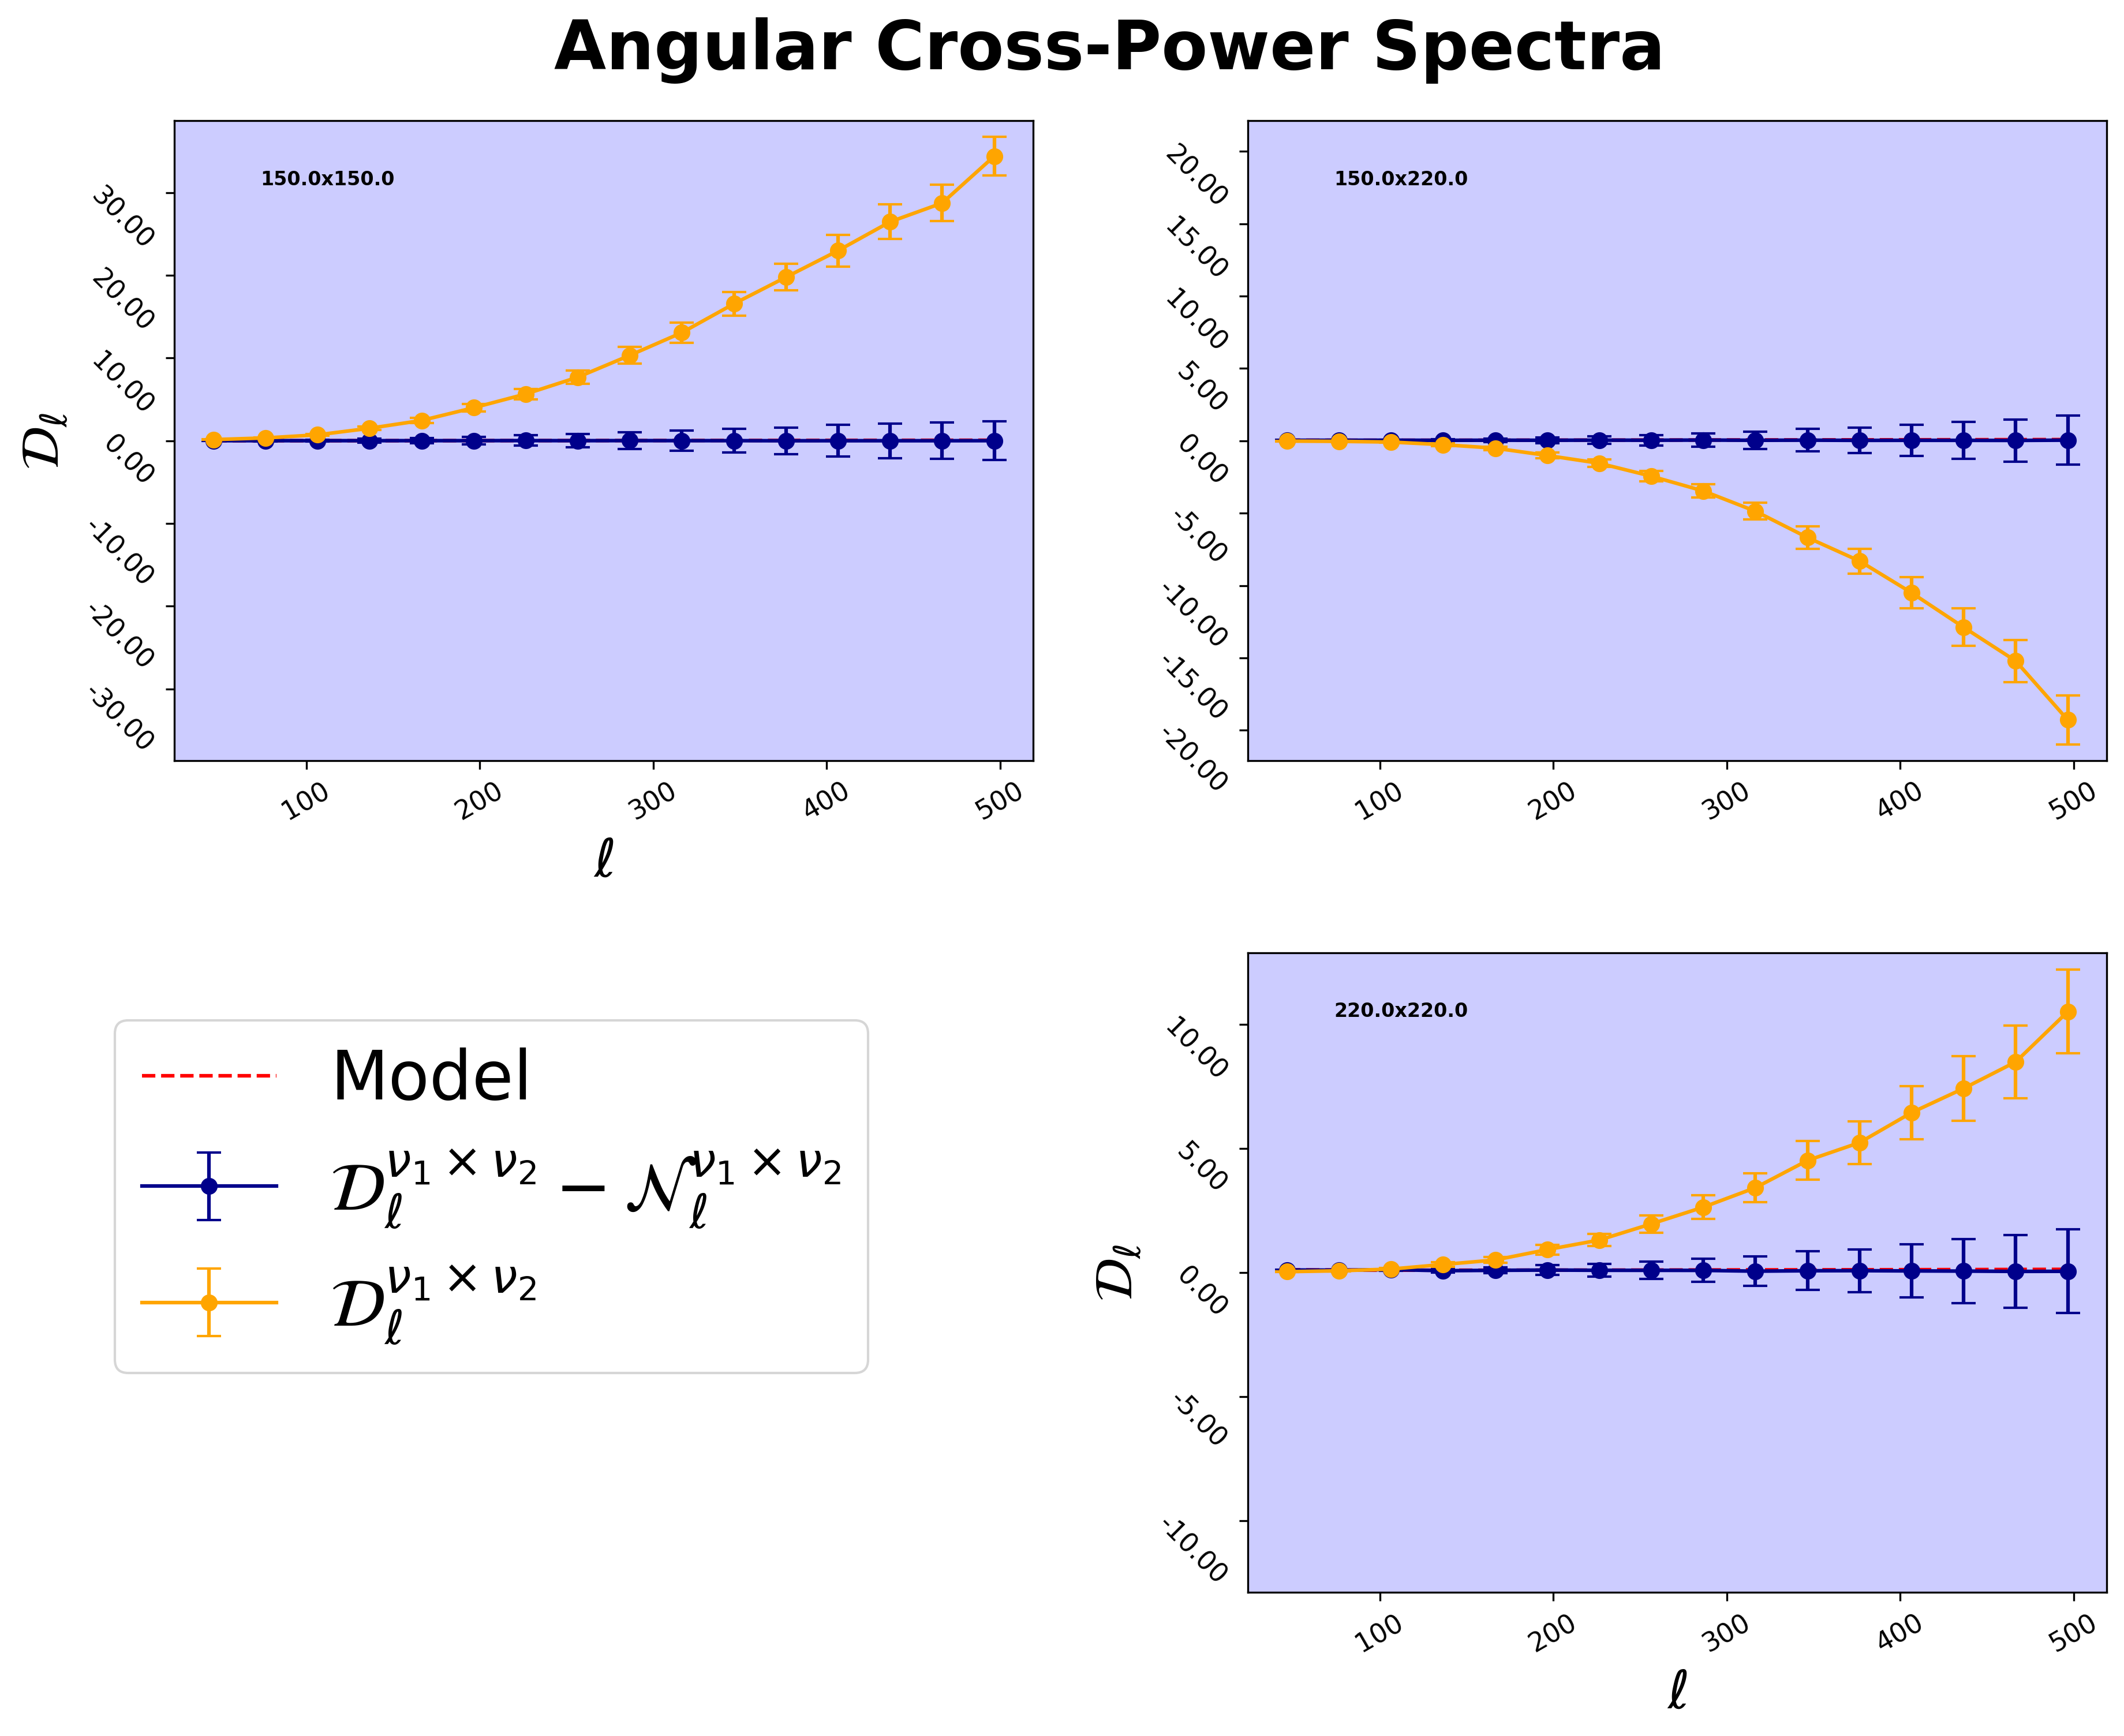
\includegraphics[width=1\linewidth]{xspectra_unbiasing_w_noise.png}}
    \end{minipage}
    \hfill
    \begin{minipage}{0.5\linewidth}
        \centerline{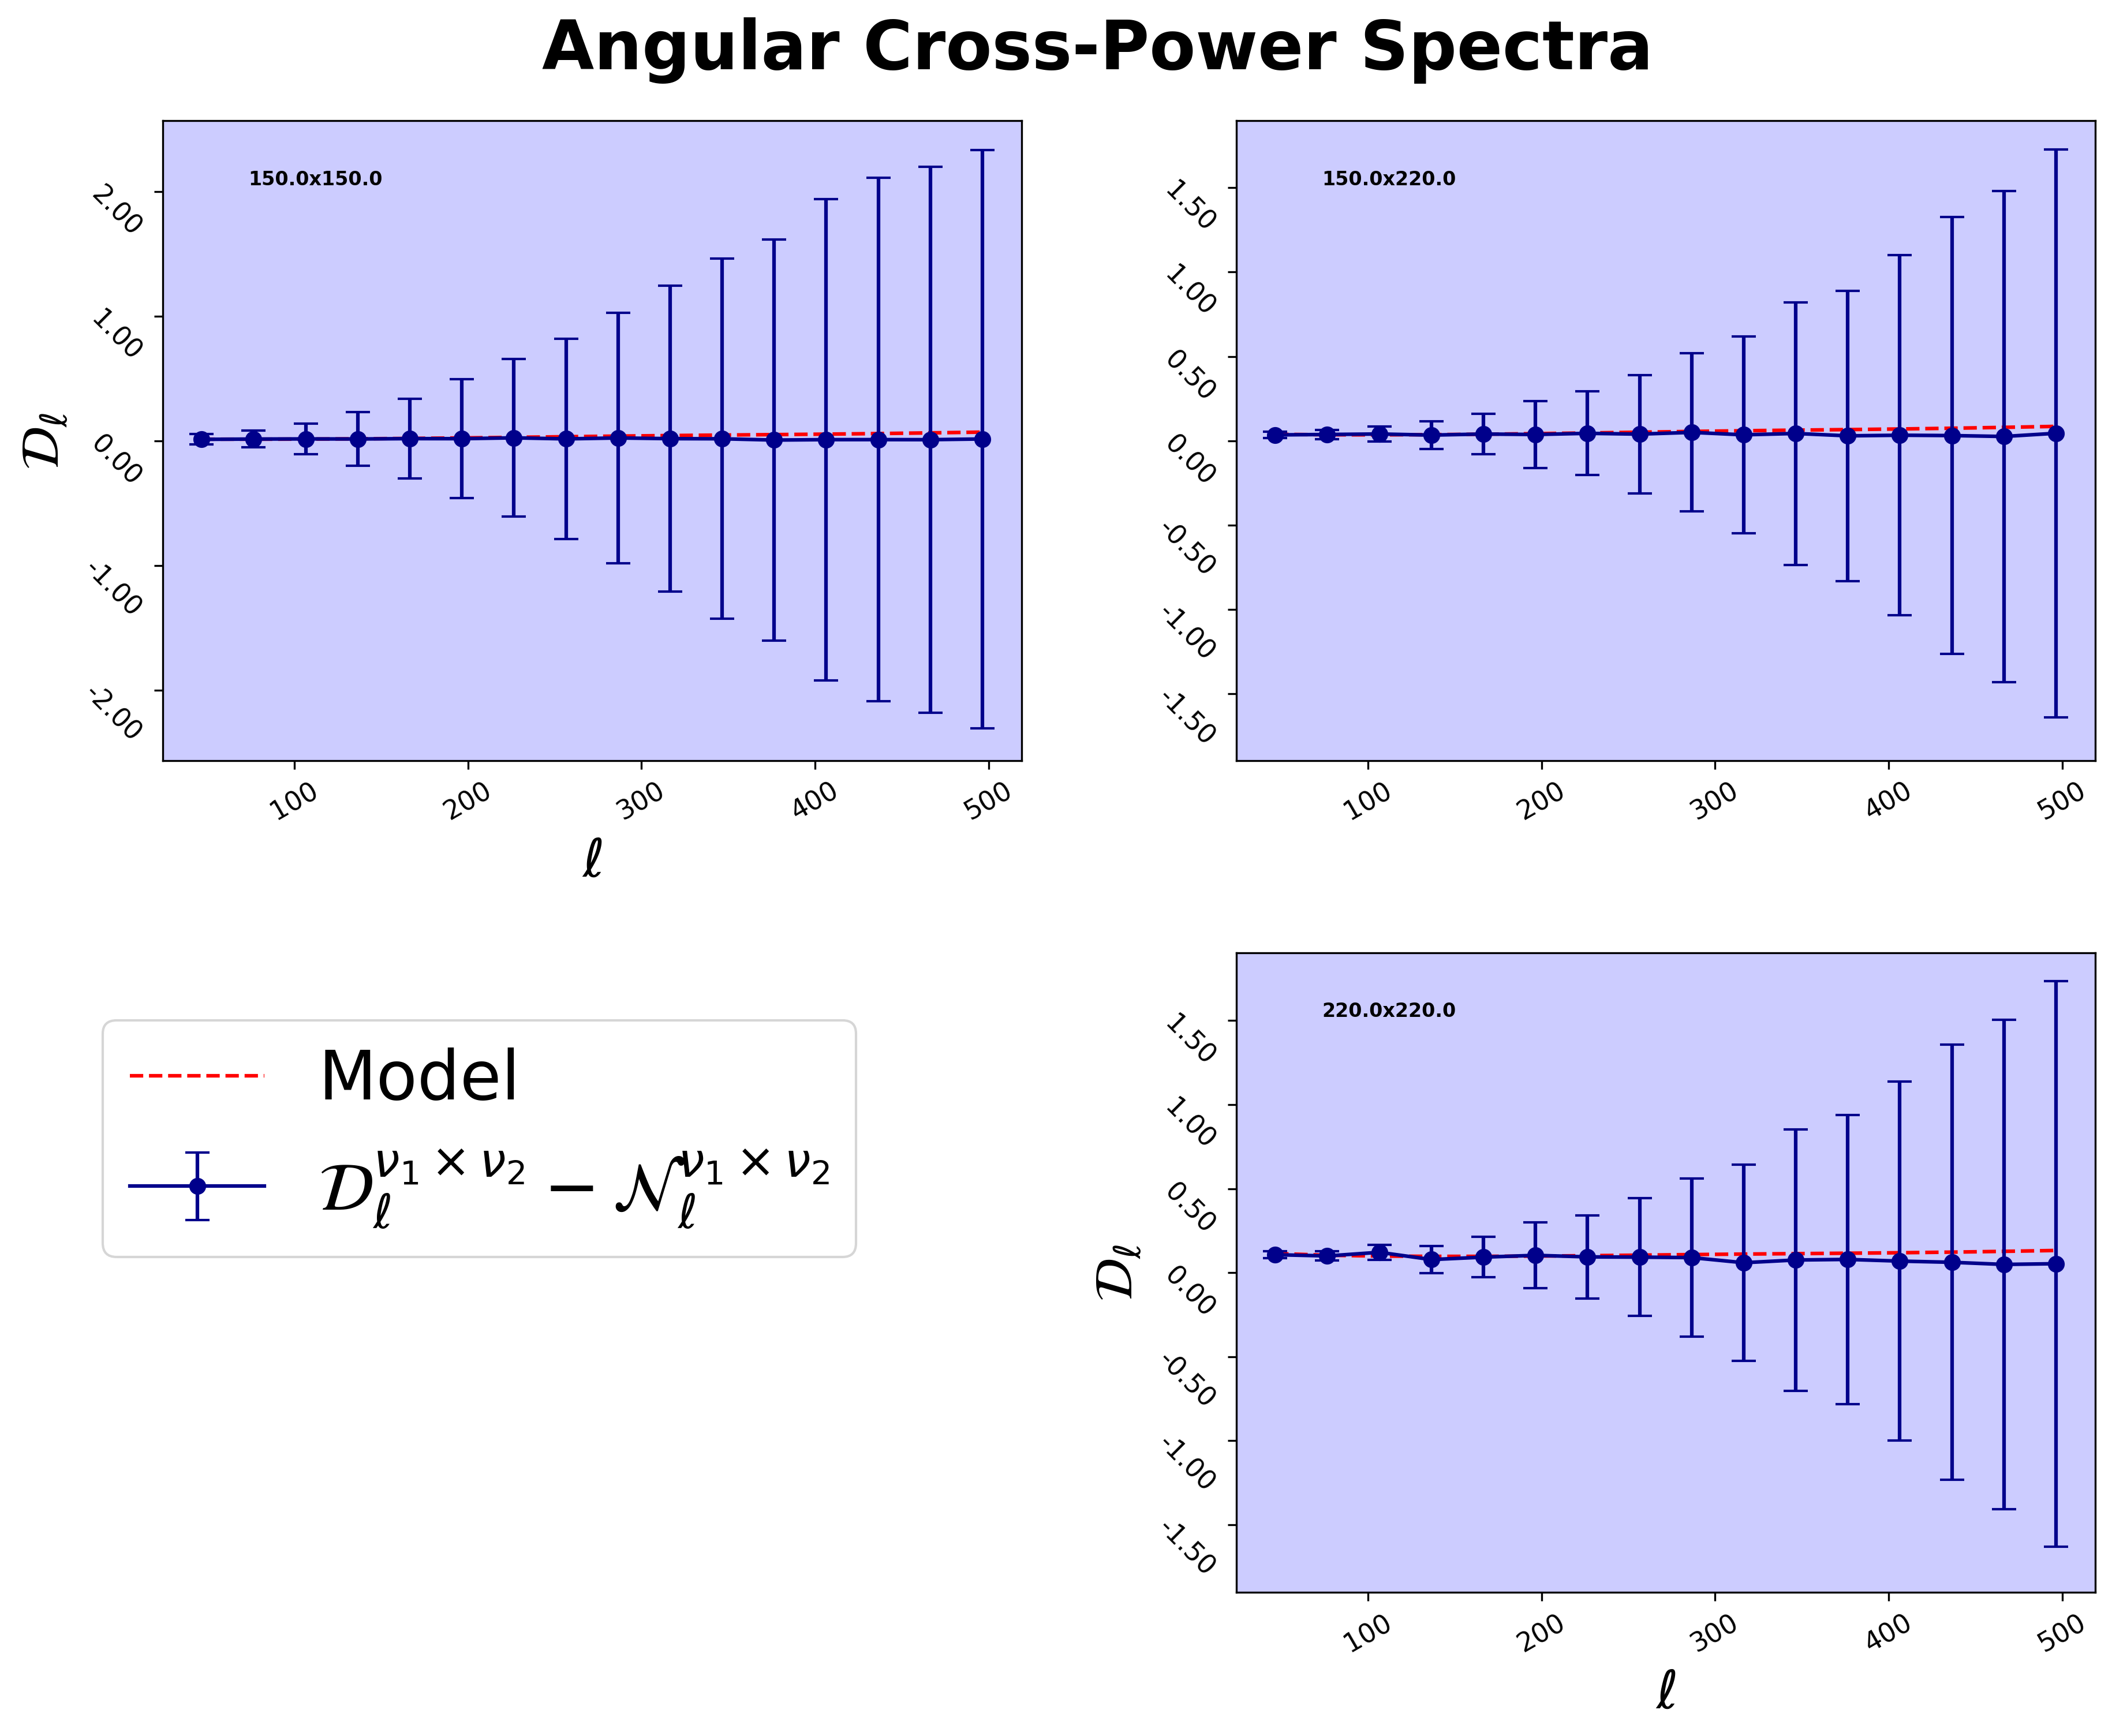
\includegraphics[width=1\linewidth]{xspectra_unbiasing_wo_noise.png}}
    \end{minipage}
    \caption{Comparison between biased and unbiased \jc{BB} cross-power spectra computed over two frequency maps. (left) The orange points are spectra containing sky signal and noise, while blue points are the spectra where we removed the noise bias. Red dash line shows the theoretical model for the signal spectra. (right) Same figure without the biased spectra, to show that the results are indeed centered around the model.}
    \label{fig:xspectra_unbiasing}
\end{figure}

\subsection{Noise covariance matrix}

To estimate the foreground and CMB parameters, we construct a noise covariance matrix that is used to weight the cost function entering the fitting procedure. Several contributions are included in this covariance matrix. The first is the covariance of the noise realisations, $Cov(N_\ell^{\mathrm{sim}})$, which is required to correctly account for the uncertainty on the measured power spectra and to debias the signal spectra. An example of the corresponding correlation matrix is shown in Figure~\ref{fig:xspectra_corr_matrix}.

\begin{figure}[!htbp]
\centering
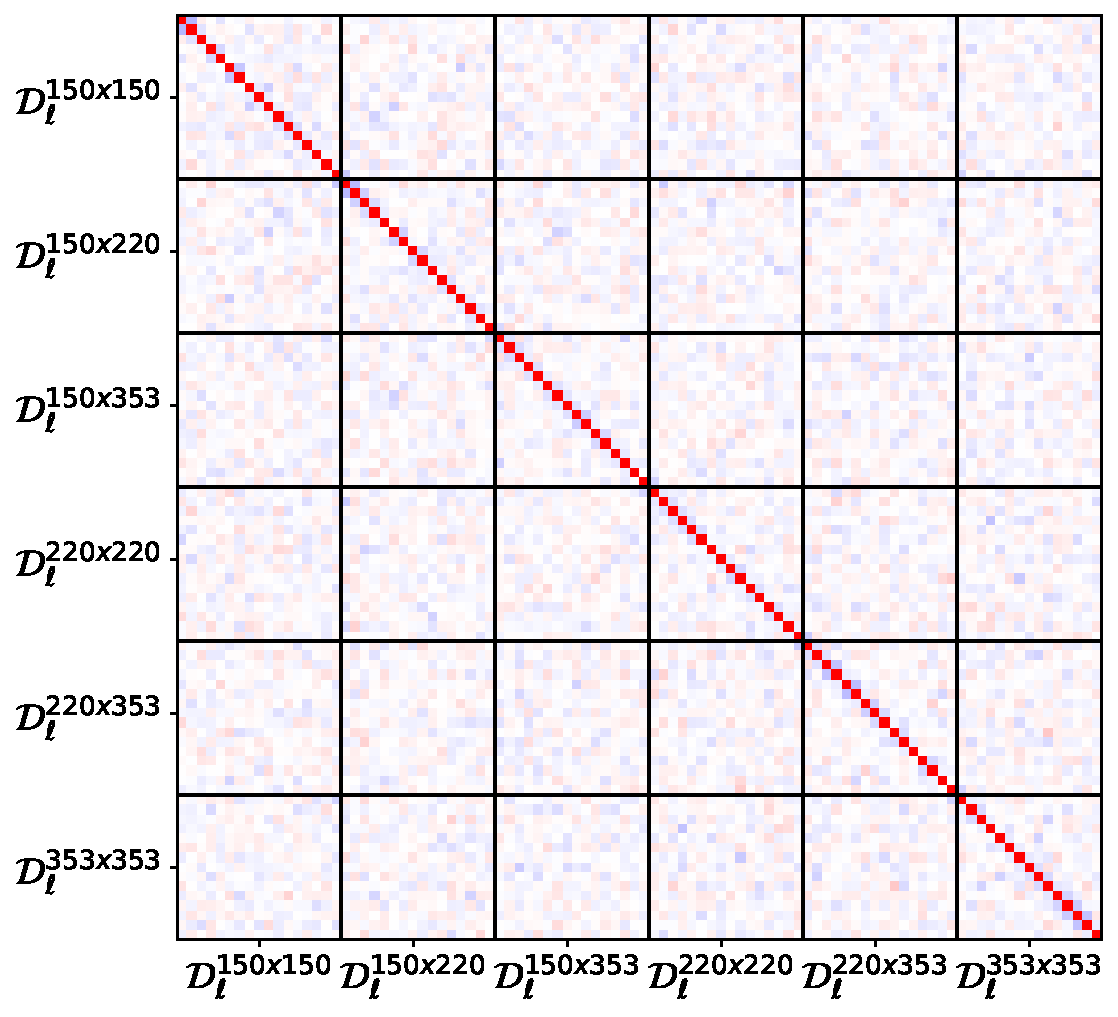
\includegraphics[width=1\linewidth]{correlation_matrix_thesis.pdf}
\caption{Correlation matrix of the cross-spectra obtained from the 150 and 220 GHz bands of QUBIC using the DB design, and the 353 GHz band of Planck. Red corresponds to a correlation coefficient of $+1$, blue to $-1$, and white to $0$. Figure taken from~\cite{FMM}. \jc{It is important to note that with spectral imaging, anti-correlations would be visible between QUBIC's frequency sub-bands.}}
\label{fig:xspectra_corr_matrix}
\end{figure}

Figure~\ref{fig:xspectra_corr_matrix} displays the correlation matrix associated with the set of auto- and cross-spectra formed from the QUBIC 150 and 220 GHz bands together with the Planck 353 GHz channel. The matrix is organised into blocks of size $(N_{\mathrm{bin}}, N_{\mathrm{bin}})$, where $N_{\mathrm{bin}}$ is the number of multipole bins. Diagonal blocks correspond to auto-spectra, while off-diagonal blocks correspond to cross-spectra between different frequency bands. The colour scale represents the correlation coefficient, with red indicating positive correlations, blue indicating negative correlations, and white indicating negligible correlations. In this example, the DB design (see Section~\ref{sub:DB_design}) is used, meaning that no spectral imaging is performed. Consequently, the QUBIC 150 and 220 GHz maps are reconstructed independently and exhibit no correlation with each other, which is reflected in the corresponding off-diagonal blocks of the matrix.

Additionally, the statistical uncertainty associated with the observation, the \emph{sample variance}, must be taken into account. In general statistical terms, sample variance refers to the uncertainty arising when a random quantity is estimated from a finite number of realisations or measurements.
In the specific context of CMB analysis, several contributions can be distinguished. The first, intrinsic contribution is the \emph{cosmic variance}, which arises from the fact that the CMB is a Gaussian random field and that we observe only a single realisation of it. For the CMB angular power spectrum, the corresponding expression for cosmic variance is given in Eq.~\ref{eq:cosmic_variance}. Additional contributions to the sample variance arise from the limited sky coverage of the observation, which reduces the number of accessible modes, as well as from the binning of the angular power spectrum in multipole space.

Therefore, we need to compute the covariance between the cross-spectra. First, we consider the cross-spectrum estimator :

\begin{equation}
    \xspec{\ell}{i}{j} = \frac{1}{2\ell+1} \sum_{m=-\ell}^{\ell} a^{\nu_i}_{\ell m}\, a^{\nu_j\,*}_{\ell m}.
\end{equation}

The covariance between two cross-spectra is defined as :
\begin{equation}
    \mathrm{Cov}\!\left(\xspec{\ell}{i}{j}, \xspec{\ell'}{k}{l}\right) = \bigl\langle \xspec{\ell}{i}{j}\,\xspec{\ell'}{k}{l} \bigr\rangle - \bigl\langle \xspec{\ell}{i}{j} \bigr\rangle \bigl\langle \xspec{\ell'}{k}{l} \bigr\rangle.
\end{equation}

Expanding the estimators gives :
\begin{align}
    \mathrm{Cov}\!\left(\xspec{\ell}{i}{j}, \xspec{\ell'}{k}{l}\right)
    &= \frac{1}{(2\ell+1)(2\ell'+1)} \sum_{m=-\ell}^{\ell} \sum_{m'=-\ell'}^{\ell'} \Big( \left\langle a^{\nu_i}_{\ell m} a^{\nu_j\,*}_{\ell m} a^{\nu_k}_{\ell' m'} a^{\nu_l\,*}_{\ell' m'} \right\rangle \nonumber\\ 
    &\qquad - \left\langle a^{\nu_i}_{\ell m} a^{\nu_j\,*}_{\ell m} \right\rangle \left\langle a^{\nu_k}_{\ell' m'} a^{\nu_l\,*}_{\ell' m'} \right\rangle \Big).
\end{align}

Assuming Gaussianity, Wick’s theorem~\cite{wick1950} gives :

\begin{align}
    \left\langle a^{\nu_i}_{\ell m} a^{\nu_j\,*}_{\ell m} a^{\nu_k}_{\ell' m'} a^{\nu_l\,*}_{\ell' m'} \right\rangle = 
    &\left\langle a^{\nu_i}_{\ell m} a^{\nu_j\,*}_{\ell m} \right\rangle \left\langle a^{\nu_k}_{\ell' m'} a^{\nu_l\,*}_{\ell' m'} \right\rangle \nonumber\\ &+ \left\langle a^{\nu_i}_{\ell m} a^{\nu_k}_{\ell' m'} \right\rangle \left\langle a^{\nu_j\,*}_{\ell m} a^{\nu_l\,*}_{\ell' m'} \right\rangle \nonumber\\ 
    &+ \left\langle a^{\nu_i}_{\ell m} a^{\nu_l\,*}_{\ell' m'} \right\rangle \left\langle a^{\nu_j\,*}_{\ell m} a^{\nu_k}_{\ell' m'} \right\rangle.
\end{align}

The first term cancels the disconnected part in the covariance definition. For a statistically isotropic field, the harmonic coefficients satisfy :

\begin{equation}
    \left\langle a^{\nu_a}_{\ell m} a^{\nu_b\,*}_{\ell' m'} \right\rangle
    = \xspec{\ell}{a}{b}\,\delta_{\ell\ell'}\,\delta_{mm'}.
\end{equation}

Using this, only the cross-pairings survive, yielding :

\begin{align}
    \mathrm{Cov}\!\left(\xspec{\ell}{i}{j}, \xspec{\ell'}{k}{l}\right)
    &= \frac{1}{(2\ell+1)(2\ell'+1)} \sum_{m,m'} \delta_{\ell\ell'}\,\delta_{mm'} \Big( \xspec{\ell}{i}{k}\,\xspec{\ell}{j}{l} + \xspec{\ell}{i}{l}\,\xspec{\ell}{j}{k} \Big).
\end{align}

The Kronecker deltas enforce $\ell=\ell'$ and $m=m'$, so that :
\begin{equation}
    \sum_{m,m'} \delta_{mm'} = \sum_{m=-\ell}^{\ell} 1 = 2\ell+1.
\end{equation}

Finally, we obtain : 
\begin{equation}
    \mathrm{Cov}\!\left(\xspec{\ell}{i}{j}, \xspec{\ell'}{k}{l}\right) = \frac{\delta_{\ell\ell'}}{2\ell+1} \left( \xspec{\ell}{i}{k}\,\xspec{\ell}{j}{l} + \xspec{\ell}{i}{l}\,\xspec{\ell}{j}{k} \right).
\end{equation}

This computation gives the covariance between two cross-spectra, but we also need to account for the limited sky coverage and the binning of spectra. Accounting for these elements, and expressing the covariance of the $D_\ell$ gives : 

\begin{equation}
    \mathrm{Cov}\!\left(\xspec{\ell}{i}{j}, \xspec{\ell'}{k}{l}\right) = \frac{\delta_{\ell\ell'}}{(2\ell+1)f_\text{sky}\Delta_\ell} \left( \xspec{\ell}{i}{k}\,\xspec{\ell}{j}{l} + \xspec{\ell}{i}{l}\,\xspec{\ell}{j}{k} \right).
\end{equation}

The resulting covariance matrix is : 

\begin{equation}
    \boxed{
    \begin{aligned}
        \text{Cov}\left(N_{\ell}^{\nu_i \times \nu_j,\,\text{sim}}, N_{\ell'}^{\nu_k \times \nu_l,\,\text{sim}}\right) &= \text{Cov}\left(N_{\ell}^{\nu_i \times \nu_j,\,\text{noise}}, N_{\ell'}^{\nu_k \times \nu_l,\,\text{noise}}\right) \\
        &+ \frac{\delta_{\ell \ell'}}{\left( 2 \ell + 1\right) f_{\text{sky}} \Delta_\ell} \left( \mathcal{D}_{\ell}^{\nu_i \times \nu_k} \mathcal{D}_{\ell'}^{\nu_j \times \nu_l} + \mathcal{D}_{\ell}^{\nu_i \times \nu_l} \mathcal{D}_{\ell'}^{\nu_j \times \nu_k} \right)
    \end{aligned}
    }
    \label{eq:xspec_noise_cov_matrix}
\end{equation}

\section{Cosmological parameters' estimation}


From the set of auto- and cross- spectra, the associated noise estimation from equation \ref{eq:xspec_noise_cov_matrix}, and the theoretical model defined in equation \ref{eq:xspec_model}, we perform a MCMC estimation, to estimate the CMB and foregrounds parameters. \\

\textbf{Remark.} A chapter dedicated to sensitivity forecasts for the QUBIC instrument was initially planned as part of this thesis. Its objective was to compare the different reconstruction methods and instrumental configurations under various sky models and simulation settings, in particular the parameters $N_\text{rec}$ for FMM and $N_\text{freq}$ for CMM. Unfortunately, due to time constraints, the results are still too preliminary to be included with sufficient confidence. Although the forecasting pipelines are fully implemented, further work is required to optimise their convergence and to achieve a deeper understanding of the obtained results before drawing robust scientific conclusions. 
\rmk{Small remark to say that a forecast chapter was planned, but was not included...}

\steve{Steve's proposition for the remark : Future work on this topic is needed to compare the different reconstruction methods and instrumental configurations under various sky models and simulation settings, in particular the parameters Nrec for FMM and Nfreq for CMM. Preliminary results are promising. The forecasting pipelines are fully implemented but further work is required to optimise their convergence and to achieve a deeper understanding of the obtained results before drawing robust scientific conclusions.}

\subsection{Simulation parameters}

In this section, we will use the simulation parameters estimated in Chapter \ref{chap:tod}. We simulate a full 3 years observation campaign for the QUBIC instrument, using the UWB configuration (see \ref{sub:UWB_design}). QUBIC observes its target patch of $15^\circ$, located in $(RA=0^\circ, DEC=57^\circ)$. We consider a sky composed of only CMB and Dust\footnote{It is a reasonable assumption to neglect the contribution from synchrotron inside the considered frequency range}, and we fix the amplitude of lensing $A_{\text{lens}}$ to $0$. In addition, the $147$, $213$ and $353$ GHz bands from Planck are added during the cross-spectra analysis. 

\subsection{FMM cross-spectrum}

With the Frequency Map-Making, we are computing frequency maps from QUBIC data. Thanks to spectral imaging, we are reconstructing multiple maps within the physical bandwidth. Increasing the number of maps has the effect of improving the component separation between CMB and astrophysical components, as it increases the number of spectra to fit their associated parameters. Figure~\ref{fig:fmm_UWB_sigma_r} shows an example of a triangle plot obtained by fitting $r$, $A_d$ and $\alpha_d$ on the maps cross-spectra (as seen in Figure~\ref{fig:fmm_xspectra}). The important values for QUBIC scientific goal are the tensor-to-scalar ratio and its associated uncertainty $\sigma_r$. As we are working on simulations, this value has to be compatible with the one used to generate the CMB signal ($r=0$), while $\sigma_r$ gives an estimation of the sensitivity of QUBIC instrument. 

\begin{figure}[!htbp]
\centering
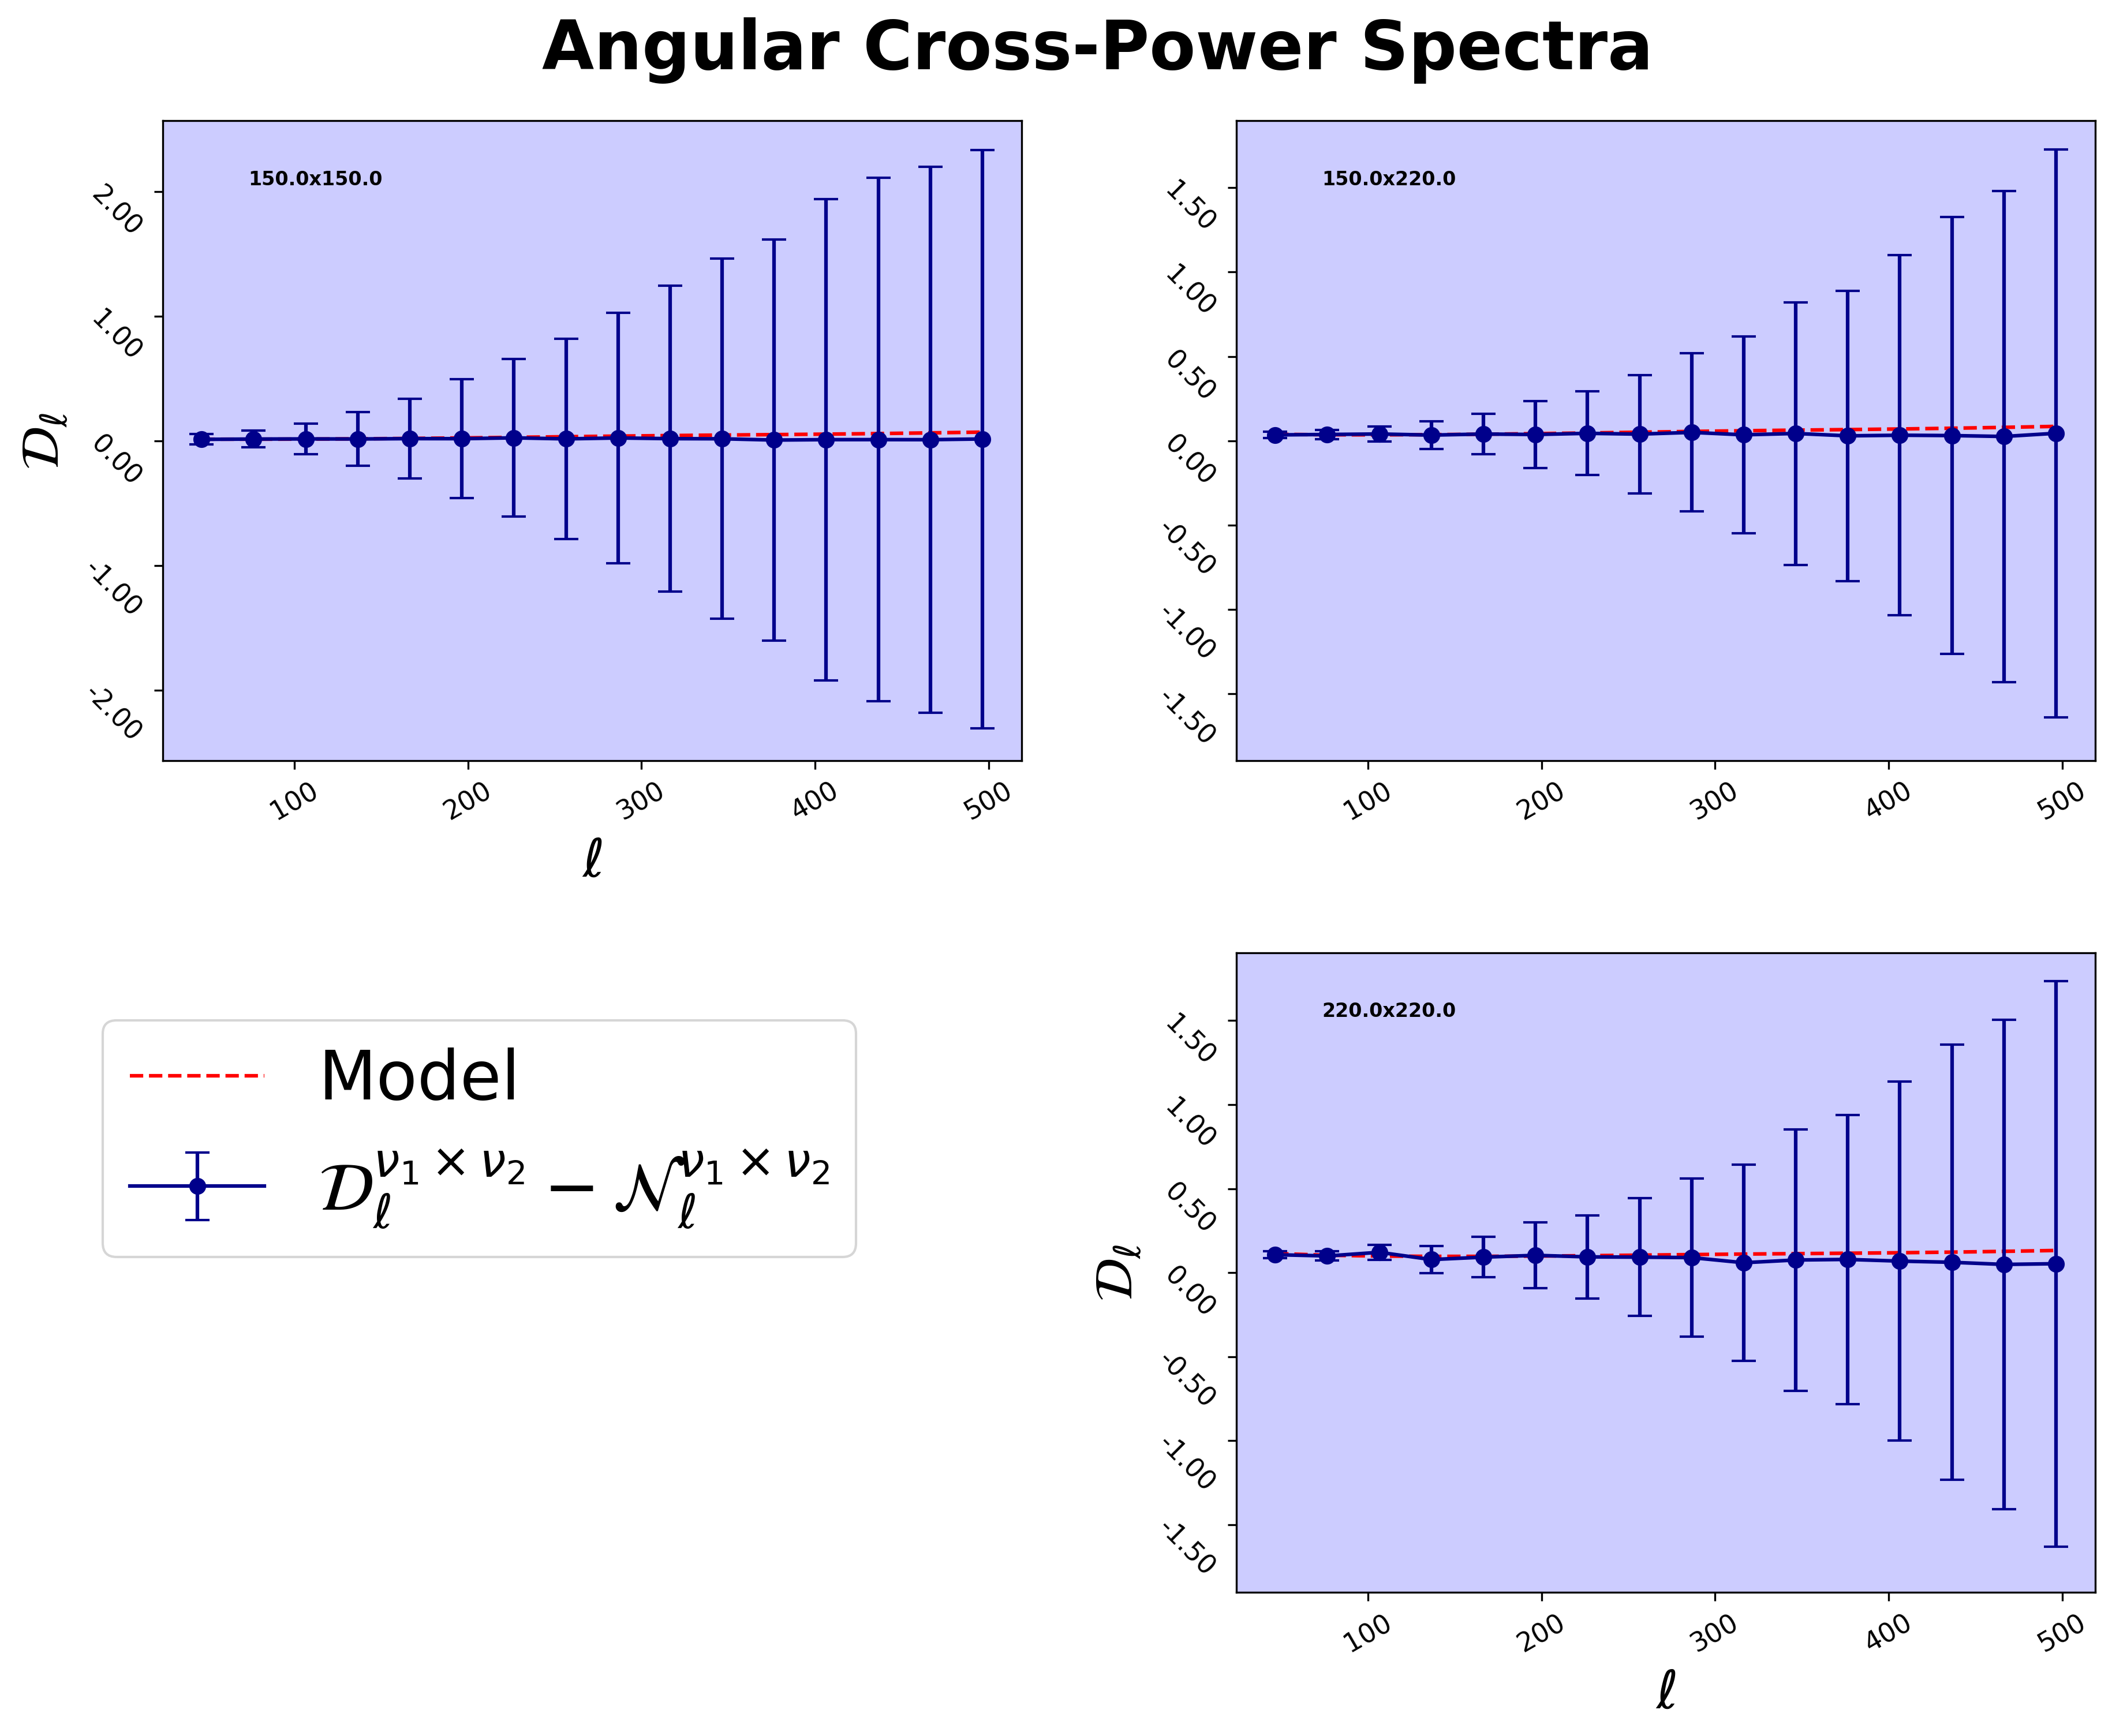
\includegraphics[width=1\linewidth]{xspectra_unbiasing_wo_noise.png}
\caption{\jc{BB} Cross-spectra computed on frequency maps obtained through FMM, with $N_\text{rec}=2$. The diagonal corresponds to the auto-spectra at $150$ and $220$ GHz, while the off-diagonal is the associated cross-spectrum.}
\label{fig:fmm_xspectra}
\end{figure}

\begin{figure}[!htbp]
\centering
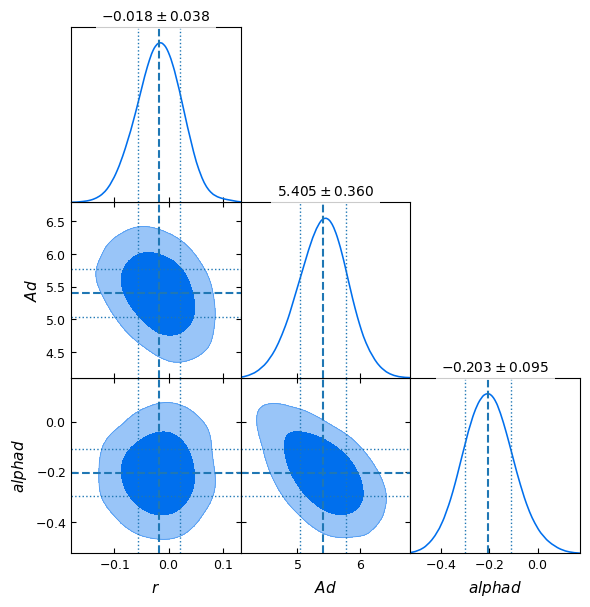
\includegraphics[width=1\linewidth]{fmm_uwb_sigma_r.png}
\caption{\tom{Triangle plot of the posterior distribution of the parameters fitted on the cross-spectra obtained with FMM.}}
\label{fig:fmm_UWB_sigma_r}
\end{figure}

\subsection{CMM cross-spectrum}

With the Component Map-Making, we are computing component maps from QUBIC data. The idea behind CMM is to perform map-making and component separation at the same time. For this purpose, two algorithms have been developed: Parametric and Blind. In both cases, the output of CMM is one map per component. In our case, it is one for CMB and one for Dust. One example of the associated cross-spectra is visible in Figure~\ref{fig:cmm_xspectra}. On the CMB auto-spectrum, we are fitting the value of $r$, while the dust parameters are estimated on the dust auto-spectrum. \jc{Because of the noise covariance between CMB and dust, due to imperfect component separation, CMB and dust parameters need to be estimated jointly.} A result of the associated fit is shown in Figure~\ref{fig:cmm_UWB_sigma_r}. 

\begin{figure}[!htbp]
\centering
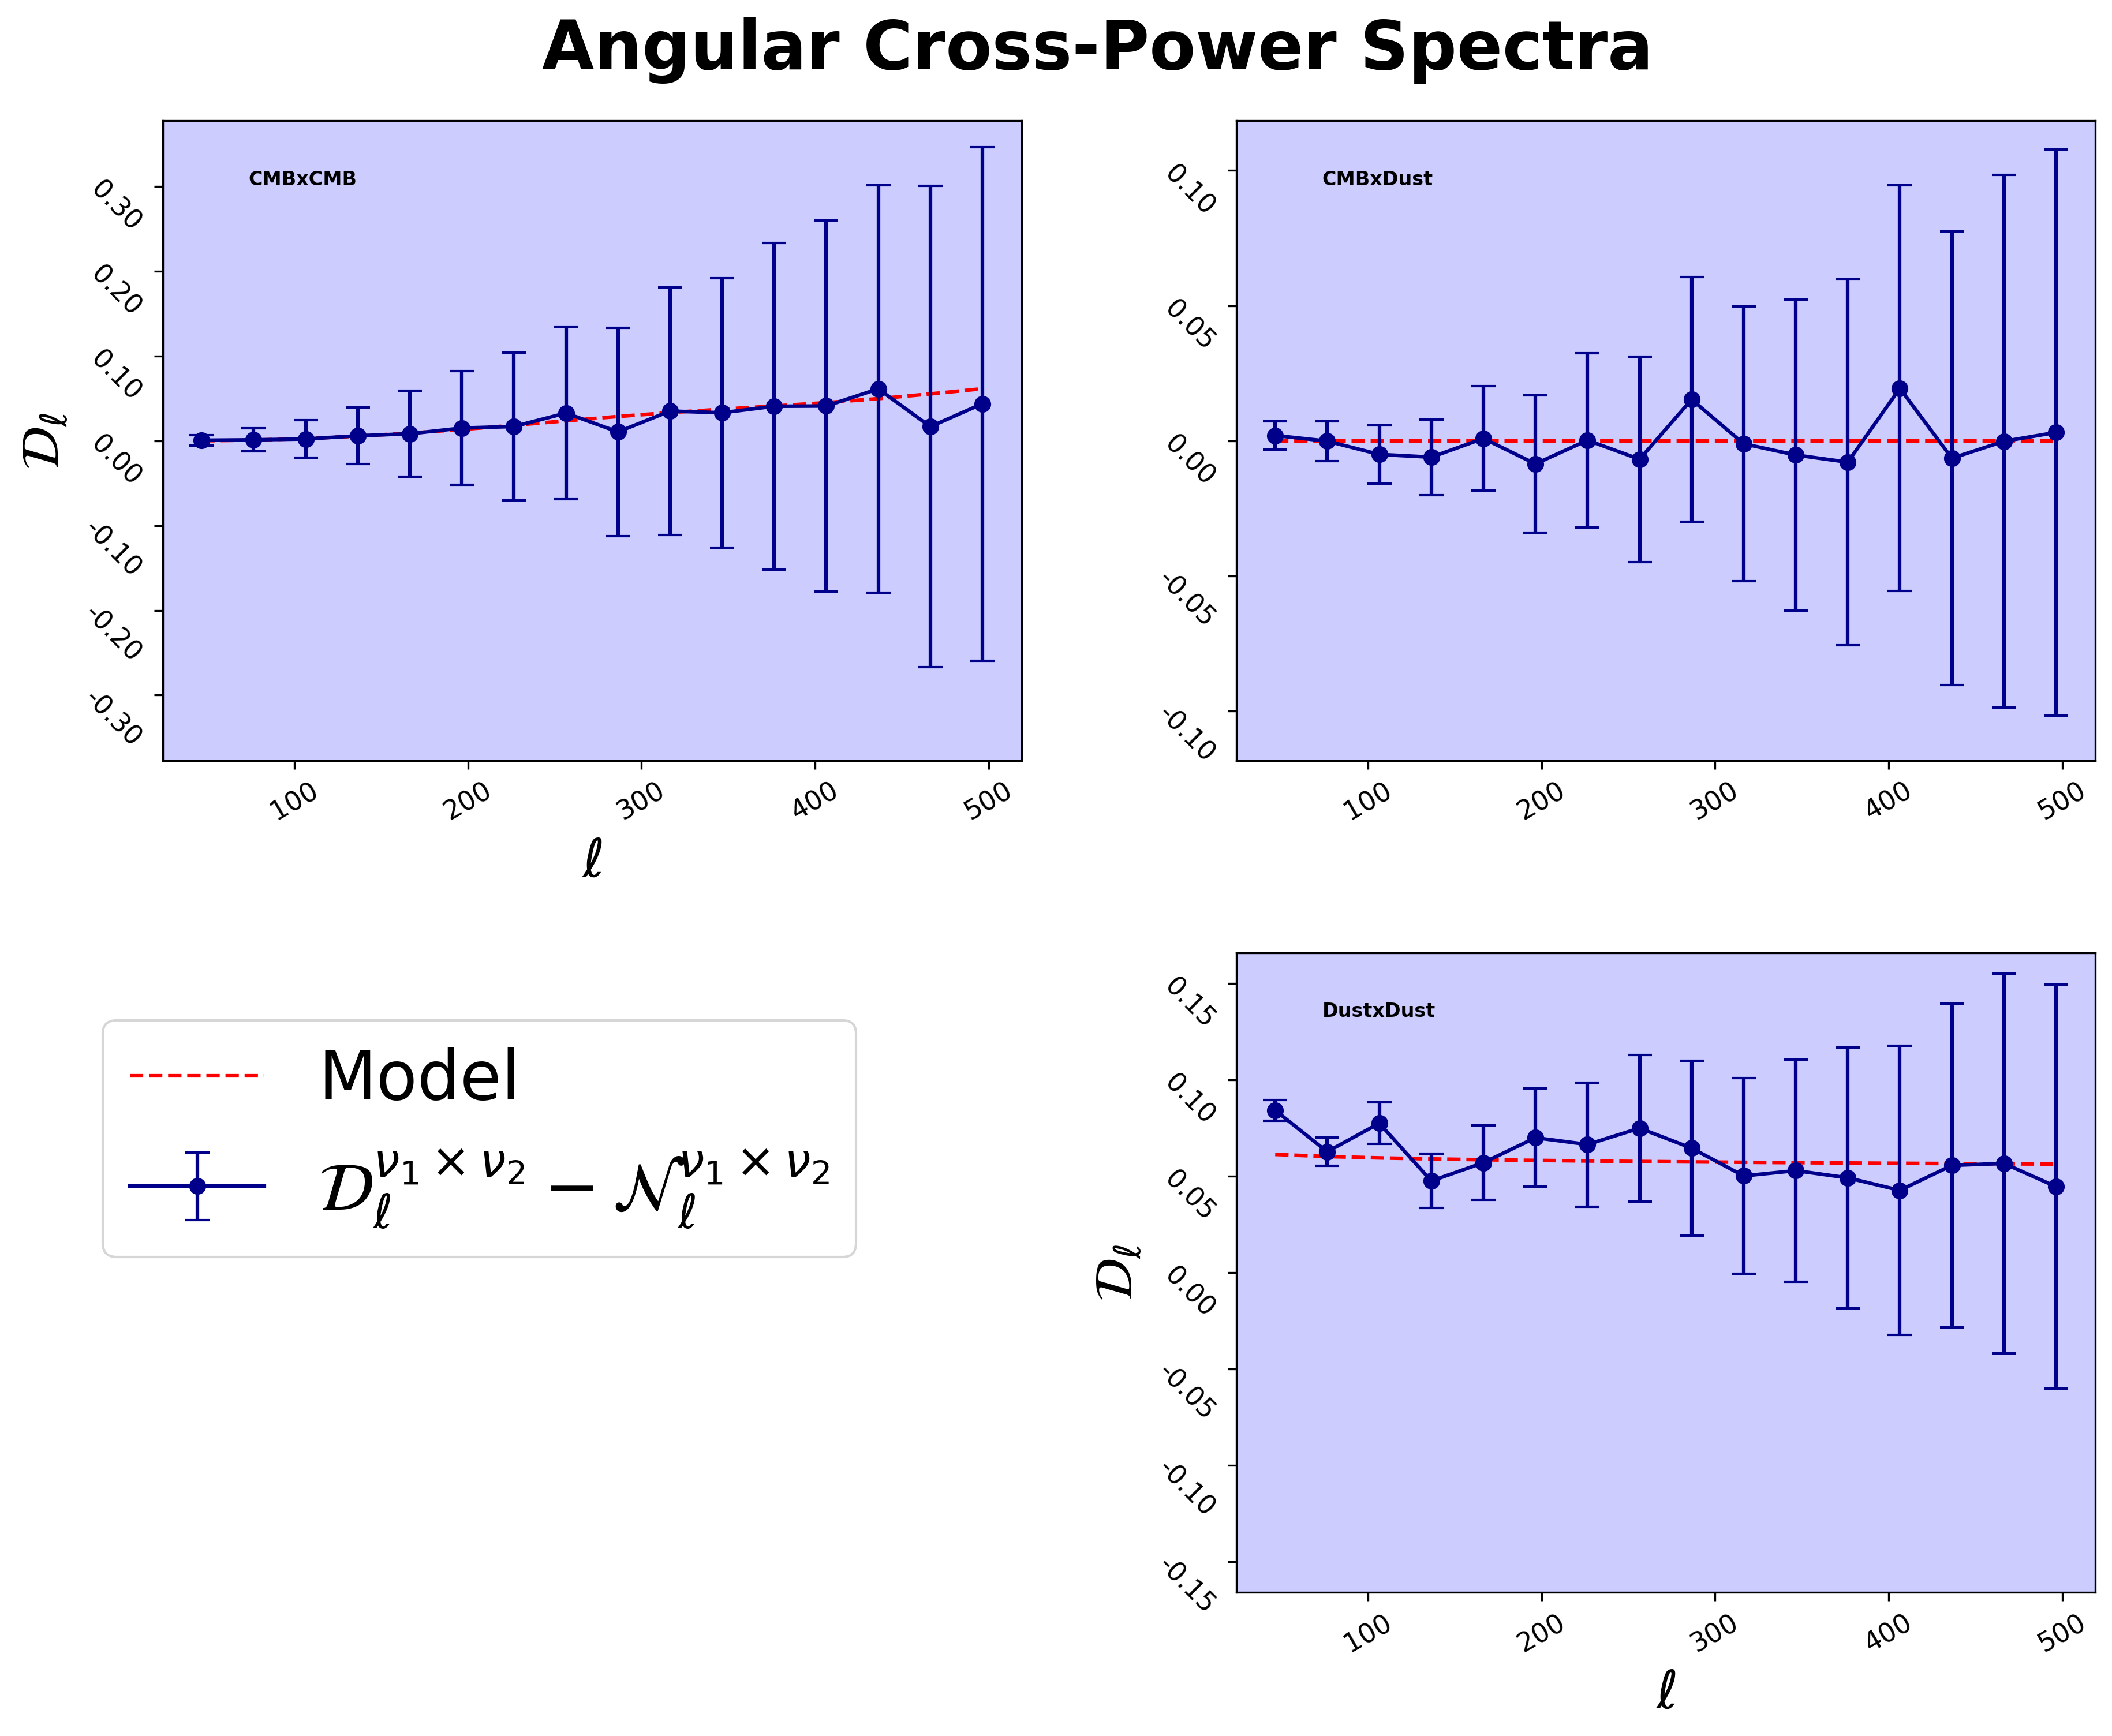
\includegraphics[width=1\linewidth]{cmm_db_xspectra.png}
\caption{\jc{BB} Cross-spectra computed on component maps obtained through CMM. The diagonal corresponds to the auto-spectra of CMB and Dust map, while the off-diagonal is the associated cross-spectrum.}
\label{fig:cmm_xspectra}
\end{figure}

\begin{figure}[!htbp]
\centering
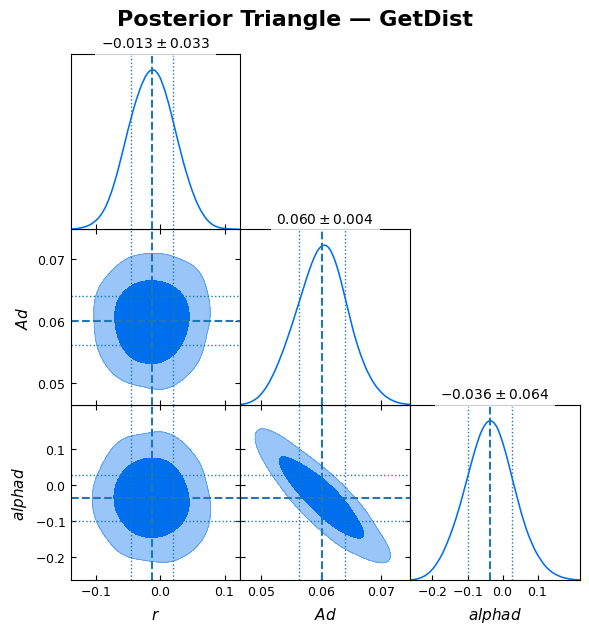
\includegraphics[width=1\linewidth]{cmm_db_sigma_r.png}
\caption{\jc{Triangle plot of the posterior distribution of the parameters fitted on the cross-spectra obtained with CMM. In this plot, the reference frequency for dust emission is $150$ GHz, instead of the most common $353$ GHz.}}
\label{fig:cmm_UWB_sigma_r}
\end{figure}


\subsection{Noise realisations}

A key aspect of the noise debiasing procedure is determining the number of noise realisations required to accurately estimate the noise contribution to the angular power spectra. Since there is no straightforward way to predict this number \emph{a priori}, we performed a series of end-to-end simulations using different numbers of noise realisations. For each configuration, the parameter estimation procedure was repeated, and the resulting constraints were analysed.
If the number of noise realisations is insufficient, the estimated noise bias may not converge to its true value, potentially leading to biased parameter estimates, including the reconstructed value of $r$. The objective is therefore to determine the minimum number of realisations for which the recovered parameters become stable.

We observed that the number of noise realisations required for convergence appears to depend on the number of frequency maps included in the fit. A possible explanation is that increasing the number of frequency channels provides additional constraints on the model parameters through a larger set of auto- and cross-spectra. As a result, the fit becomes more sensitive to small inaccuracies in the estimated noise bias. For example, using five frequency maps leads to fifteen auto- and cross-spectra\footnote{The number of spectra scales as $N_{\mathrm{freq}}(N_{\mathrm{freq}}+1)/2$.}, while only a few parameters are fitted. In such a highly constrained configuration, residual biases in the estimated spectra are more easily detected by the likelihood than in a fit involving only two frequency maps. Consequently, a larger number of noise realisations may be required to achieve convergence. Further investigation would nevertheless be needed to fully understand and quantify this effect.

To investigate this effect, we performed the analysis on simulations containing only CMB signal and noise, thereby avoiding additional complications related to component separation. The results are summarised in Figure~\ref{fig:Nreal}.
The upper panel shows the fitted value of the tensor-to-scalar ratio $r$ together with its associated uncertainty, obtained from an MCMC analysis. The fit was repeated using different numbers of noise realisations, $N_{\mathrm{real}} = [50, 100, 200, 500, 1000]$. Triangular markers indicate cases where the recovered value is not statistically compatible with the true input value, $r=0$, revealing a residual bias in the debiasing procedure. The analysis was performed in three different configurations. The blue points correspond to a fit using only the two QUBIC frequency bands, $150$ and $220$~GHz, in the DB configuration. The orange points correspond to the same QUBIC bands supplemented by the Planck $143$, $217$, and $353$~GHz channels. Finally, the green points include the full set of seven Planck frequency channels in addition to the two QUBIC bands. The lower panel displays the corresponding uncertainty on the fitted tensor-to-scalar ratio, $\sigma_r$, as a function of $N_{\mathrm{real}}$. Crosses identify configurations for which the recovered value of $r$ is not compatible with the true input value.

A clear dependence on the number of frequency channels can be observed. The three configurations do not require the same number of noise realisations to achieve a stable and unbiased estimate of $r$. When only the two QUBIC bands are included, approximately $100$ noise realisations are sufficient. Adding the three Planck channels increases this requirement to roughly $300$ realisations. Finally, when all nine frequency channels are considered, more than $500$ realisations are needed before the recovered value becomes compatible with the input one. These results support the hypothesis that increasing the number of frequency channels makes the fit more sensitive to small inaccuracies in the estimated noise bias.

\begin{figure}[!htbp]
    \centering
    
\includegraphics[width=1\linewidth]{n_real.png}
    \caption{Recovered tensor-to-scalar ratio $r$ (top) and corresponding uncertainty $\sigma_r$ (bottom) as a function of the number of noise realisations used in the debiasing procedure. The three colours correspond to different sets of frequency channels included in the fit. Triangles and crosses indicate configurations for which the recovered value of $r$ is not statistically compatible with the input value $r=0$.}
    \label{fig:Nreal}
\end{figure}

\jc{The observed behaviour can be explained by the fact that the inverse of an unbiased estimator of the covariance matrix is not, in general, an unbiased estimator of the inverse covariance matrix~\cite{taylor2013}. Consequently, as the dimensionality of the covariance matrix increases, a larger number of realisations is required to obtain an approximately unbiased estimate of its inverse.}


\end{document}